\documentclass[a4paper,12pt]{scrartcl}

\usepackage[ngerman]{babel} % Neue Deutsche Rechtschreibung
\usepackage[utf8]{inputenc} % utf-8 Eingabe
\usepackage[T1]{fontenc}
\usepackage{csquotes}
\setcounter{tocdepth}{10} % Aufnahme in das Inhaltsverzeichnis *
\setcounter{secnumdepth}{10} % Nummerierungslevel vertiefen
\usepackage{hyperref}
\newcommand\fnurl[2]{%
	\href{#2}{#1}\footnote{\url{#2}}%
}
\usepackage{graphicx}
\graphicspath{{/figuren/}}

\begin{document}
	
	\begin{titlepage}
		\centering
		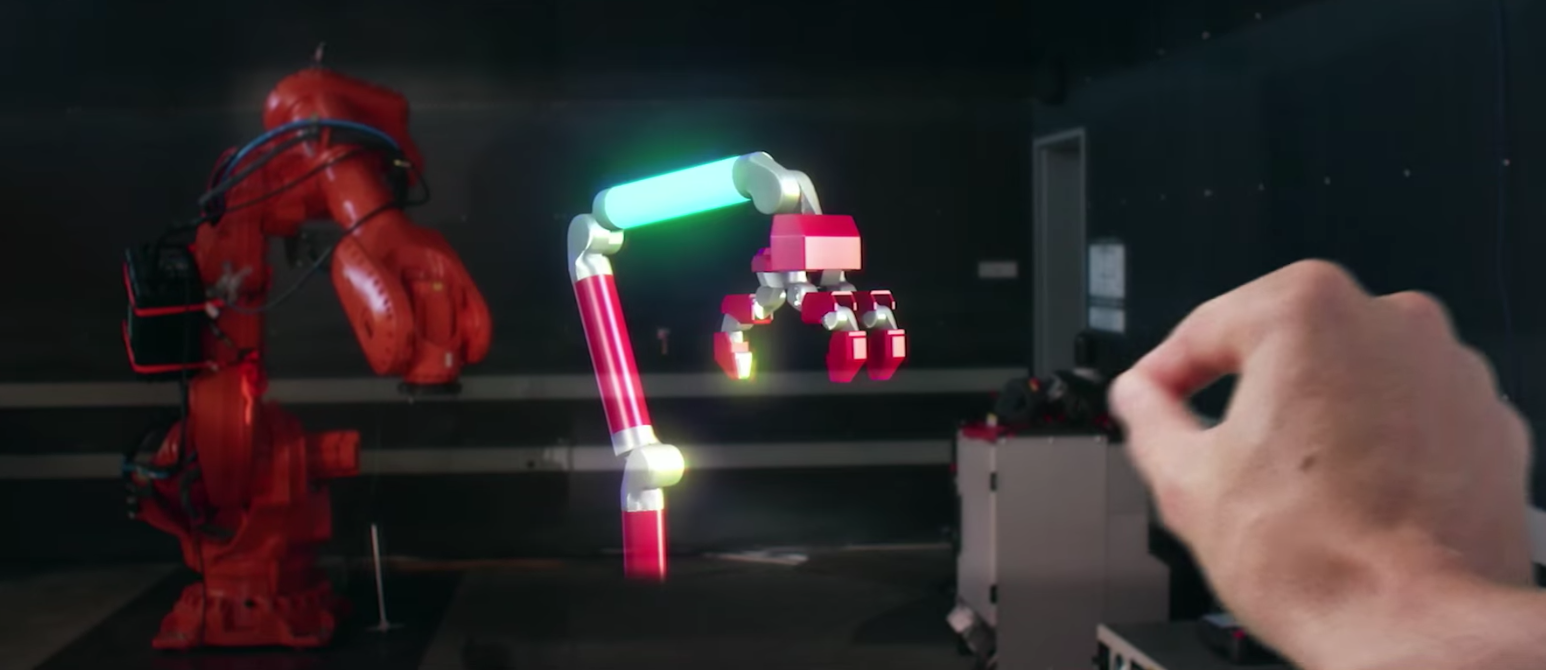
\includegraphics[width=1.0\textwidth]{figuren/HoloLens_CompanyVideo_2016_11_24_10_13_20}\par\vspace{1cm}
		{\scshape\LARGE Beuth Hochschule für Technik Berlin \par}
		\vspace{1cm}
		{\scshape\Large Praxisbericht\par}
		\vspace{1.5cm}
		{\huge\bfseries Konzeption und prototypische Implementierung von innovativen Interaktionen mit Industriemaschinen im virtuellen Raum im Kontext Industrie 4.0\par}
		\vspace{2cm}
		{\Large\itshape Ibrahim Khaled Reguieg\par}
		\vfill
		betreut von\par
		Prof. Dr. Dipl.-Ing. Kristian \textsc{Hildebrand}
		
		Dr. Dipl.-Ing. Joachim \textsc{Quantz}
		\vfill	
	\end{titlepage}
	
	\tableofcontents
	
	\newpage
	\topskip0pt
	\vspace*{\fill}
	\begin{quote}
		"Das gesamte Universum ist keine Maschine, die man in Einzelteile zerlegen kann wie ein Auto, sondern ein gigantisches multidimensionales Hologramm."
		
		- David Bohm 
	\end{quote}
	\vspace*{\fill}
	\newpage

\section{Einleitung}
An der Beuth Hochschule für Technik Berlin ist im sechsten Semester des Medieninformatik Bachelorstudiums eine Praxisphase von dreimonatiger Dauer angesetzt. Sie soll die Bacheloranden darauf vorbereiten, wie das Arbeitsleben als Entwickler in der freien Wirtschaft nach dem Abschluss aussehen könnte und Inspiration für selbigen geben. So ist es gewünscht, die Praxisphase in einem profitorientierten Unternehmen zu vollziehen, um erstens technologisch, als auch strategisch, das Geschehen am Puls der Zeit wahrnehmen zu können. Die Praxisphase liegt, im Studiengang Medieninformatik, selben Semester wie der Abschluss selbst. So verkürzt teilt sich das sechste Semester in drei Monate Praxisphase und drei Monate Bearbeitungszeit für die Abschlussarbeit selbst. So kommt es, dass auch ich, in der finalen Phase des Studiums angelangt, mir eine Stelle für die Praxisphase suchen muss.

\subsection{Weg zur Praktikumsstelle}
Nachdem ich mir einige Zeit darüber Gedanken machte, welche Themenfelder mich in Hinblick auf meinen Abschluss interessieren und für welche Dinge ich eine Passion pflege, kam ich zu dem Entschluss, dass die "neuen" Technologien wie Augmented- und Virtual-Reality(AR \& VR) in Verbindung mit Robotik oder Spieleentwicklung in Frage kommen. Also formulierte ich ein kleines Exposé, indem es um die fortschreitende Entwicklung und Automatisierung der Maschinen geht und wie der Mensch dieser Situation Herr bleiben kann. Dieses schickte ich meinem Professor Prof. Dr. Dipl-Ing. Hildebrand, um ihn zu fragen und davon zu überzeugen mein Betreuer bei besagtem Vorhaben zu werden. Er erachtete die Fragestellung und das zugehörige Szenario als sehr interessant und willigte ein.
\newline
\newline
Danach begann der Bewerbungsprozess für eine Stelle im Bereich VR/AR im Zuge dessen ich mich unter anderem bei, Exozet Berlin GmbH, Kinematics GmbH, Framefield GmbH und dem Frauenhofer-Institut bewarb.


Ich hatte schon fast den Vertrag bei Kinematics GmbH unterschrieben, als mir Prof. Hildebrand mitteilte, dass sein ehemaliger Arbeitgeber ART+COM Studios AG zeitnah ein neues Forschungsprojekt startet, bei dem es hauptsächlich darum gehen soll, den Leitstand einer Werksfeuerwehr mit Live-Bildern von Drohnen, die mit Informationen angereichert in einer Datenbrille visualisiert zur Verfügung gestellt werden, zu unterstützen.
\newline
\newline
Besagtes Projekt trägt den Namen Elektronisch gestützte Fernwartung für Werksfeuerwehren(EFFeu). Und da mein Exposé und meine Vorstellungen für die genannte Abschlussarbeit exakt passten, entschloss ich mich die Praxisphase bei ART+COM Studios AG zu beginnen.

\subsection{Der Praktikumsbetrieb}
%\subsection{Das Unternehmen ART+COM AG}
Die ART+COM Studios ist seit 1998 eine nicht börsennotierte AG, getragen von den ehemaligen Mitgliedern des ART+COM e.V., Mitarbeitern und dem Vorstand. Letzterer wird gebildet von Andreas Wiek und Prof. Joachim Sauter.
\newline
Das Unternehmen ist in drei Kategorien aufgeteilt:
\newline
\newline
ART+COM ART gestaltet mediale Skulpturen und Installationen, die auf ihre jeweiligen Orte wirken und ihnen – über ihre Funktion und ihre Architektur hinaus – Identität geben. Unsere Kunstprojekte entstehen sowohl im Auftrag für den öffentlichen Raum als auch in eigenem Auftrag.

ART+COM COMMUNICATION entwirft und realisiert mediale Installationen und Räume, die komplexe Inhalte gezielt vermitteln und Information erlebbar machen. Wir gestalten Exponate für Ausstellungen, Museen und Markenräume.

ART+COM RESEARCH erforscht die neuen Medien und ihre Anwendungsmöglichkeiten sowohl unabhängig als auch in Kooperation mit Unternehmen und akademischen Institutionen.

Das circa 60 Personen umfassende Team besteht zum größten Teil aus festangestellten Mitarbeitern, die sich in circa zwei Viertel Gestalter, ein Viertel Entwickler und ein Viertel Buchhaltung und Geschäftsleitung aufteilen. Außerdem werden weitere Kompetenzen durch freie Mitarbeiter ergänzt.

\section{Tätigkeitsbereich und Aufgaben}

Mein Tätigkeitsbereich bei ART+COM bezieht sich auf drei Hauptaufgabenbereiche, die alle im Bereich Entwicklung liegen:
\newline
\newline
- VR Showcases von Kunstinstallationen mit Unity
- AR Showcases für Kunden mit Unity
- Shader in Unity

Zunächst startete erwartungsgemäß die Einarbeitungsphase, bei der ich mich in die Technologien Unity Pro, SteamVR Plugin und SteamVR Toolkit einarbeitete. Dies befähigt mich Applikationen für HTCs Virtual Reality Headset Vive mit Unity Pro zu bauen.
Im späteren Verlauf der Praxisphase folgten weitere Technologien. Das Microsofts HoloLens, welche mit einem Set an Tools, dass sich HoloToolkit nennt und ShaderLab, um Unity Shader für eine 16K aufgelöste Panorama-Videowand, und zukünftig hoffentlich etliche, Projekte entwickeln zu können.

\subsection{Überblick}
Mein Kommilitone Chris, der sein Praktikum ebenfalls, allerdings zwei Wochen zeitversetzt, bei ART+COM absolviert und ich haben unser Büro im 6. OG des Bürogebäudes am Wittenbergplatz. Der Raum trägt den Namen Holodeck und die beiden high-performance Windows 10 Rechner, auf welchen wir entwickeln, tragen folgerichtig die Namen holodeck1 und holodeck2. Die beiden Maschinen sind mit ihren Grafikarten der neusten Generation, nVidia Gefore GTX 980Ti und 1080 VR-Ready. Eine  Voraussetzung, die zum Ausführen und Entwickeln von VR Applikationen erfüllt sein muss. Da für VR fähige Head Mounted Displays(HMD) zeitgleich zwei stereoskopische Kamerabilder gerendert werden müssen, für jedes Auge eines, ist die Belastung der Grafikeinheit des Rechners sehr hoch. So kommt es, dass man zusätzlich zum VR Headset noch einen Rechner, der über genügend Perfomance verfügt benötigt.

Die Entwicklungsabteilung von Art+Com entwickelt agil und mit den entsprechenden Methoden SCRUM und KANBAN.

\subsection{Das EfFeu-Projekt}
\subsection{Entwickeln für VR/AR/MR}
Da, wie bereits erwähnt, für VR fähige Head Mounted Displays(HMD) zwei stereoskopische Kamerabilder gerendert werden müssen und deswegen die Belastung der Grafikeinheit sehr hoch ist, ist bei Multimedia-Anwendungen im virtuellen Raum, beispielsweise, das Abspielen eines hoch aufgelösten Films, durchaus mit FPS-Drops, Glitches oder gar Abstürtzen zu rechnen. Die Performanceoptimierung im Bereich VR ist nach wie vor ein sehr wichtiges und aktuelles Thema. vgl. LinkZu10KMethode oder Unity VR Performance Update.
\subsubsection{Geschichte}
VR und auch AR sind keineswegs neue Technologien.
VR hatte sein Debüt schon in den 1990er Jahren. Die potenziellen Anwendungsfälle und Visionen haben sich seitdem im großen und ganzen kaum verändert, allerdings und das haben wir hauptsächlich dem technologischen Fortschritt im Sinne von Moore's Law zu verdanken, ist der Einstieg in den Consumermarket heutzutage durchaus gegeben. Brauchte man früher noch die finanzielle Kapazität einer ganzen Forschungseinrichtung und Rechenmaschinen, die ganze Gebäudetrakte füllten, um eine Anwendung mit mäßiger computergrafischen Leistung stereoskopisch zu Rendern und in die Datenbrille zu übertragen, bedarf es heutzutage nur noch eines performanten Gaming-Rechners und dem Headset seiner Wahl, ganz zu schweigen von den VR - Lösungen à la Cardboard und der gleichen, die nur mit Hilfe eines Smartphones begrenzte, aber durchaus würdige VR-Erlebnisse darstellen können.
\subsubsection{Devices und ihre Vor- und Nachteile}
\paragraph{Virtual Reality}
Als virtuelle Realität bezeichnet man einen Raum, im, dessen Projektion stereoskopisch, auf zwei vor den Augen angebrachten Bildschirmen, gerendert wird.
3D-Objekte können in diesem Raum ohne Probleme dargestellt werden, und sie können in all ihren Freiheitsgraden translatiert, rotiert, skaliert und vor allem auch betrachtet werden. Im Gegensatz zu herkömmlichen Spielen, die sich mit dem Zusatz 3D schmückten, wird in der Welt des VR ein echtes dreidimensionales Gefühl entwickelt, da durch Headtracking mit Gyroskopsensor, Infrarottracking im realen Raum und stereoskopischem Rendering eben dieses Gefühl nahezu real wirkt.

So bekommt ein Anwender das Gefühl tatsächlich im virtuellen Raum anwesend zu sein.
\subparagraph{Smartphonehalterungen}
Inzwischen kann man so ziemlich jedes Smartphone, welches zur neueren Generation zählt, ganz einfach in ein HMD umfunktionieren. Diverse Hersteller bieten, zum Teil sehr kostengünstige, Lösungen an, bei denen man das Smartphone vor zwei Linsen spannt und diese in Verbindung mit einer VR App den Bildschirm auf die zwei Linsen optimiert aufteilen. Da das Smartphone bereits über Lagesensoren, Gyroskop und Display verfügt braucht es nur die zusätzlichen Linsen plus Halterung, um eine einigermaßen ansprechende VR Erfahrung zu gewährleisten.

Es existieren bereits unzählige Lösungen, allen voran Googles Cardboard und Samsungs GearVR.
\subparagraph{Oculus Rift}
Die Rift genannte HMD vom Hersteller Ocolus, welcher 2015 von Facebook für die beachtliche Summe von 6 Milliarden US-Dollar gekauft wurde, war der erste große Aufschrei in der "neuen" Welt des VR. Sie starteten mit einer Kickstarter Kampagne und hatten schon nach wenigen Stunden das Mindestziel erreicht. Das Headset erschien in drei Versionen. Development Kit 1, Development Kit 2 und Consumer Version.
\subparagraph{HTC Vive}
HTCs Konkurrenzprodukt zu Oculuss Rift kam in etwa zeitgleich, wie das Rift auf den Markt.
\paragraph{Augmented Reality}
\subparagraph{Smartphonelösungen}
\subparagraph{Industriebrillen}
\subparagraph{Microsoft HoloLens}
\subsubsection{Entwicklertools}
\subsubsection{Lizenzierung und professionelles Entwickeln}

\begin{thebibliography}{1}
	
	\bibitem{notes} Ph.D. Jerald, Jason (2016): {\em The VR Book.} 1. Aufl., ACM Books, San Rafael
	
	\bibitem{impj}  The Japan Reader {\em Imperial Japan 1800-1945} 1973:
	Random House, N.Y.
	
	\bibitem{norman} E. H. Norman {\em Japan's emergence as a modern
		state} 1940: International Secretariat, Institute of Pacific
	Relations.
	
	\bibitem{fo} Bob Tadashi Wakabayashi {\em Anti-Foreignism and Western
		Learning in Early-Modern Japan} 1986: Harvard University Press.
	
\end{thebibliography}


\end{document}